\chapter{The Seated Hope Stamps}

\section{The Second Definitive Issue 'Retouched Die' the Outer Line Removed}

\heading{(1871-1876)}

As the old dies started to wear out the printers Messrs De La Rue \& Co. 
requested to have the original dies altered by removing the outer line frame. 
In addition they had the shading upon the figure of Hope and the vine 
leaves redrawn.

With the exception of the Six Pence and One Shilling stamps which 
retained the outer frame line.


\begin{marginfigure}
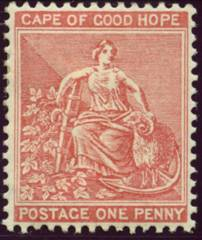
\includegraphics[width=1.0\textwidth]{../cape-of-good-hope/clip_image002_0002.jpg}
\caption{
Retouched Die Showing the Outer Frame Line Removed
}
\end{marginfigure}

\begin{marginfigure}
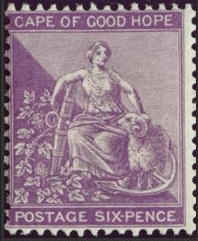
\includegraphics[width=1.0\textwidth]{../cape-of-good-hope/clip_image002_0001.jpg}
\caption{
Original Die Showing the Outer Frame Line (You can see the frame easier 
if you look at the bottom of the stamp)
}
\end{marginfigure}

It appears that De La Rue wrote to the Crown Agents on July 12, 1870 
reasoning that the firm was againt the stamps having thin frame lines
as these could be damaged and wear easily1. The letter has not survived but
the Crown Agent's reply of July 13th did and we quote:

\begin{quotation}
Referring to your letter of the 12th instant respecting the renewal
of the Cape of Good Hope postage plate, duty 1d., I have to acquaint
you that the Crown Agents consent to the preparation of a new forme
at a cost of \pounds85, as well as you altering the die in the
manner proposed.
\end{quotation}

The new plate of 240 multiples was invoiced on October 26, 1870, and the next
supply of One Penny stamps was invoiced on June 8, 1871, when 687,120 were charged.


\section{The Five Shillings Stamp}

\heading{(Issued prior to 25th August 1871)}
 
In February 1871 the Postmaster General reported the need for a 
higher duty stamp. His reason for his recommendation was that 
owing to the fact that several One Shilling stamps were necessary 
to frank a single letter inconvenience has been experienced through 
the covering up of the front of the envelopes and the concealment 
of the addresses. In addition difficulty arose by the stamps being 
detached in the post.
This was accepted and the die and stamps were prepared by Messrs. 
De La Rue and Co. The order for the die and the plate for the
Five Shillings came on March 27, 1871 as part of a routine order
for reprints of the One Penny, Foupence and One Shilling. The
choice of colour was left to De La Rue. The die and a plate
of 240 multiples was invoiced on June 5th. (Easton, p290).


The first consignment amounted to 100 sheets of 240 stamps each. 
These were despatched from England by the s.s. Roman on the 9th June 1871. 
They reached Cape Town about the 17th July.They were issued to the public 
towards the end of August 1871.

\subsubsection{Printings}

Several subsequent printings of the Five Shillings stamps upon the 
paper watermarked with the Crown CC were made. Noticeable shades 
of the orange-yellow are obtainable.


\section{Deepening of the 4d shade to a darker blue.}

Easton writes (p 295) that deepening of the shade of blue of the Cape of Good Hope
Fourpence with frame line was intentional. When sending their requisition for a further supply on January 9, 1872 the Crown Agents wrote:

\begin{quotation}
The local Postmaster suggests that, if practicable, the four penny stamps should be tinted a shade deeper than heretofore, as by gaslight the colour of the stamp assumes
a greenish hue, and is therefore liable to be mistaken for the 1/- label which
is light green.
\end{quotation}

The firm in their acknowledgement of January 10th then suggested `that if a little
black were mixed with blue ink, as shown on the enclosed specimen' there would be
sufficient contrast. The specimen was approved January 13th. 




1. Easton, p287. 



                                                                                                              